\documentclass[border=12pt]{standalone}
\usepackage{tikz}
\usetikzlibrary{arrows}
\begin{document}
  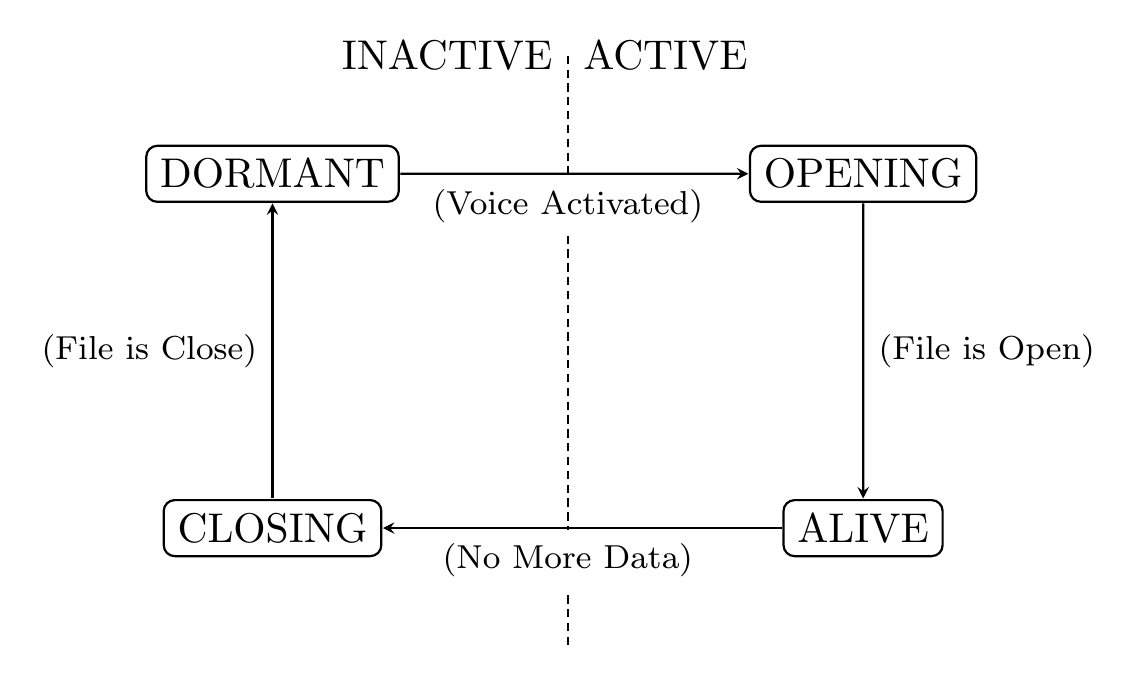
\begin{tikzpicture}[
      scale = 1.5, transform shape, thick,
      Line/.style = {draw, -stealth},
      State/.style = {draw, rectangle, fill = white, rounded corners},
      StateChange/.style = {fill = white, font = \footnotesize}
    ]
    \node at (1,5) [State](A){DORMANT};
    \node at (6,5) [State](B){OPENING};
    \node at (6,2) [State](C){ALIVE};
    \node at (1,2) [State](D){CLOSING};

    \path [Line] (A) -- (B);
    \path [Line] (B) -- (C);
    \path [Line] (C) -- (D);
    \path [Line] (D) -- (A);

    \draw[densely dashed]   (3.5,6) node[left]{INACTIVE} node[right]{ACTIVE} -- (3.5,1);

    \node[StateChange, below] at (3.5,5) {(Voice Activated)};
    \node[StateChange, below] at (3.5,2) {(No More Data)};
    \node[StateChange, left] at (1, 3.5) {(File is Close)};  
    \node[StateChange, right] at (6, 3.5) {(File is Open)};  
  \end{tikzpicture}
\end{document}
